\begin{center}
\begin{figurehere}
\begin{tikzpicture}[line cap=round,line join=round,>=triangle 45,x=0.7cm,y=0.7cm]
%x-akseli:
\draw[->,color=gray] (-2.5,0) -- (3.5,0);
%tiksut ja viivat
\foreach \x in {,-2,-1,1,2,3}
{\draw[dashed, color= lightgray] (\x,-2.5)--(\x,4.5);
\draw[shift={(\x,0)},color=black] (0pt,1pt) -- (0pt,-1pt);
}
\node [below] at (3.5,0) {$x$};

%y-akseli
\draw[->,color=gray] (0,-2.5) -- (0,4.5);
%tiksut ja viivat
\foreach \y in {-2,-1,1,2,3,4}
{
\draw[dashed, color=lightgray] (-2.5,\y)--(3.5,\y);
\draw[shift={(0,\y)},color=black] (1pt,0pt) -- (-1pt,0pt);
}
\node [left] at (0,4.5) {$y$};

% Varsinainen kuva
\draw[thick] (-1.75,-2.5)--(1.75,4.5);
\node[above left] at (-2,4) {C};
\end{tikzpicture}
\end{figurehere}
\end{center}

%kuva 2

\begin{center}
\begin{figurehere}
\begin{tikzpicture}[line cap=round,line join=round,>=triangle 45,x=0.7cm,y=0.7cm]
%x-akseli:
\draw[->,color=gray] (-2.5,0) -- (3.5,0);
%tiksut ja viivat
\foreach \x in {,-2,-1,1,2,3}
{\draw[dashed, color= lightgray] (\x,-2.5)--(\x,4.5);
\draw[shift={(\x,0)},color=black] (0pt,1pt) -- (0pt,-1pt);
}
\node [below] at (3.5,0) {$x$};

%y-akseli
\draw[->,color=gray] (0,-2.5) -- (0,4.5);
%tiksut ja viivat
\foreach \y in {-2,-1,1,2,3,4}
{
\draw[dashed, color=lightgray] (-2.5,\y)--(3.5,\y);
\draw[shift={(0,\y)},color=black] (1pt,0pt) -- (-1pt,0pt);
}
\node [left] at (0,4.5) {$y$};

% Varsinainen kuva
\draw[thick] (-2.5,-1.75)--(3.5,1.25);
\node[above left] at (-2,4) {B};
\end{tikzpicture}
\end{figurehere}
\end{center}
	
%kuva 3

\begin{center}
\begin{figurehere}
\begin{tikzpicture}[line cap=round,line join=round,>=triangle 45,x=0.7cm,y=0.7cm]
%x-akseli:
\draw[->,color=gray] (-2.5,0) -- (3.5,0);
%tiksut ja viivat
\foreach \x in {,-2,-1,1,2,3}
{\draw[dashed, color= lightgray] (\x,-2.5)--(\x,4.5);
\draw[shift={(\x,0)},color=black] (0pt,1pt) -- (0pt,-1pt);
}
\node [below] at (3.5,0) {$x$};

%y-akseli
\draw[->,color=gray] (0,-2.5) -- (0,4.5);
%tiksut ja viivat
\foreach \y in {-2,-1,1,2,3,4}
{
\draw[dashed, color=lightgray] (-2.5,\y)--(3.5,\y);
\draw[shift={(0,\y)},color=black] (1pt,0pt) -- (-1pt,0pt);
}
\node [left] at (0,4.5) {$y$};

% Varsinainen kuva
\draw[thick] (-2.5,4.5)--(3.5,-1.5);
\node[above left] at (-1,4) {A};
\end{tikzpicture}
\end{figurehere}
\end{center}

%kuva 4
\begin{center}
\begin{figurehere}
\begin{tikzpicture}[line cap=round,line join=round,>=triangle 45,x=0.7cm,y=0.7cm]
\draw[fill, color= LightSkyBlue] (0,0)--(6,0)--(6,1.5)--(0,1.5)--cycle;
\draw (0,0)--(6,0)--(6,4)--(0,4)--cycle;
\foreach \y in {1,...,7}
{
\draw (0,0.5*\y)--(6,0.5*\y);
}

\end{tikzpicture}
\hspace{1cm}
\begin{tikzpicture}[line cap=round,line join=round,>=triangle 45,x=0.7cm,y=0.7cm]
\draw[fill, color= LightSkyBlue] (0,0)--(5,0)--(5,4)--(0,4)--cycle;
\draw (0,0)--(6,0)--(6,4)--(0,4)--cycle;
\foreach \x in {1,...,5}
{
\draw (\x,0)--(\x,4);
}

\end{tikzpicture}
\end{figurehere}
\end{center}

%kuva 5
\begin{center}
\begin{figurehere}
\begin{tikzpicture}[line cap=round,line join=round,>=triangle 45,x=0.7cm,y=0.7cm]
\draw[fill, color= LightSkyBlue] (0,0)--(6,0)--(6,1.5)--(0,1.5)--cycle;
\draw (0,0)--(6,0)--(6,4)--(0,4)--cycle;
\foreach \y in {1,...,7}
{
\draw (0,0.5*\y)--(6,0.5*\y);
}
\foreach \x in {1,...,5}
{
\draw (\x,0)--(\x,4);
}
\end{tikzpicture}
\hspace{1cm}
\begin{tikzpicture}[line cap=round,line join=round,>=triangle 45,x=0.7cm,y=0.7cm]
\draw[fill, color= LightSkyBlue] (0,0)--(5,0)--(5,4)--(0,4)--cycle;
\draw (0,0)--(6,0)--(6,4)--(0,4)--cycle;
\foreach \x in {1,...,5}
{
\draw (\x,0)--(\x,4);
}
\foreach \y in {1,...,7}
{
\draw (0,0.5*\y)--(6,0.5*\y);
}
\end{tikzpicture}
\end{figurehere}
\end{center}

%kuva 6
\begin{center}
\begin{figurehere}
\begin{tikzpicture}[line cap=round,line join=round,>=triangle 45,x=0.7cm,y=0.7cm]
\draw[fill, color= LightSkyBlue] (0,0)--(6,0)--(6,4)--(0,4)--cycle;
\draw (0,0)--(6,0)--(6,4)--(0,4)--cycle;
\foreach \y in {1,...,7}
{
\draw (0,0.5*\y)--(6,0.5*\y);
}
\foreach \x in {1,...,5}
{
\draw (\x,0)--(\x,4);
}
\end{tikzpicture}
\hspace{1cm}
\begin{tikzpicture}[line cap=round,line join=round,>=triangle 45,x=0.7cm,y=0.7cm]
\draw[fill, color= LightSkyBlue] (0,0)--(5,0)--(5,1)--(0,1)--cycle;
\draw (0,0)--(6,0)--(6,4)--(0,4)--cycle;
\foreach \x in {1,...,5}
{
\draw (\x,0)--(\x,4);
}
\foreach \y in {1,...,7}
{
\draw (0,0.5*\y)--(6,0.5*\y);
}
\end{tikzpicture}
\end{figurehere}
\end{center}

%kuva 7
\begin{center}
\begin{figurehere}
\begin{tikzpicture}[line cap=round,line join=round,>=triangle 45,x=0.7cm,y=0.7cm]
\draw[fill, color= LightSkyBlue] (0,0)--(6,0)--(6,4)--(0,4)--cycle;
\draw (0,0)--(6,0)--(6,4)--(0,4)--cycle;
\foreach \y in {1,...,3}
{
\draw (0,\y)--(6,\y);
}
\foreach \x in {1,...,5}
{
\draw (\x,0)--(\x,4);
}
\end{tikzpicture}
\hspace{1cm}
\begin{tikzpicture}[line cap=round,line join=round,>=triangle 45,x=0.7cm,y=0.7cm]
\draw[fill, color= LightSkyBlue] (0,0)--(5,0)--(5,1)--(0,1)--cycle;
\draw (0,0)--(6,0)--(6,4)--(0,4)--cycle;
\foreach \x in {1,...,5}
{
\draw (\x,0)--(\x,4);
}
\foreach \y in {1,...,3}
{
\draw (0,\y)--(6,\y);
}
\end{tikzpicture}
\end{figurehere}
\end{center}

%kuva 8 kertolasku
\begin{center}
\begin{figurehere}
\begin{tikzpicture}[line cap=round,line join=round,>=triangle 45,x=0.7cm,y=0.7cm]
\draw[fill, color= LightSkyBlue] (0,0)--(5,0)--(5,4)--(0,4)--cycle;
\draw (0,0)--(6,0)--(6,4)--(0,4)--cycle;
\foreach \x in {1,...,5}
{
\draw (\x,0)--(\x,4);
}
\end{tikzpicture}
\hspace{1cm}
\begin{tikzpicture}[line cap=round,line join=round,>=triangle 45,x=0.7cm,y=0.7cm]
\draw[fill, color= LightSkyBlue] (0,0)--(5,0)--(5,1.5)--(0,1.5)--cycle;
\draw (0,0)--(6,0)--(6,4)--(0,4)--cycle;
\foreach \x in {1,...,5}
{
\draw (\x,0)--(\x,4);
}
\foreach \y in {1,...,7}
{
\draw (0,0.5*\y)--(6,0.5*\y);
}
\end{tikzpicture}
\end{figurehere}
\end{center}

%kuva 9 kertolasku
\begin{center}
\begin{figurehere}
\begin{tikzpicture}[line cap=round,line join=round,>=triangle 45,x=0.7cm,y=0.7cm]
\draw[fill, color= LightSkyBlue] (0,0)--(3,0)--(3,1.5)--(0,1.5)--cycle;
\draw[fill, color= LightSkyBlue] (3,0)--(6,0)--(6,1)--(3,1)--cycle;
\draw (0,0)--(6,0)--(6,4)--(0,4)--cycle;
\foreach \x in {1,...,5}
{
\draw (\x,0)--(\x,4);
}
\foreach \y in {1,...,7}
{
\draw (0,0.5*\y)--(6,0.5*\y);
}
\end{tikzpicture}
\hspace{1cm}
\begin{tikzpicture}[line cap=round,line join=round,>=triangle 45,x=0.7cm,y=0.7cm]
\draw[fill, color= LightSkyBlue] (0,0)--(3,0)--(3,1.5)--(0,1.5)--cycle;
\draw[fill, color= LightSkyBlue] (3,0)--(6,0)--(6,1)--(3,1)--cycle;
\draw (0,0)--(6,0)--(6,4)--(0,4)--cycle;
\draw (3,0)--(3,4);
\foreach \y in {1,...,7}
{
\draw (0,0.5*\y)--(6,0.5*\y);
}
\end{tikzpicture}
\end{figurehere}
\end{center}

%kuva 10 jakolasku
\begin{center}
\begin{figurehere}

\begin{tikzpicture}[line cap=round,line join=round,>=triangle 45,x=0.7cm,y=0.7cm]
\draw[fill, color= LightSkyBlue] (0,0)--(6,0)--(6,1.5)--(0,1.5)--cycle;
\draw (0,0)--(6,0)--(6,4)--(0,4)--cycle;
\foreach \y in {1,...,7}
{
\draw (0,0.5*\y)--(6,0.5*\y);
}
\end{tikzpicture}
\hspace{1cm}
\begin{tikzpicture}[line cap=round,line join=round,>=triangle 45,x=0.7cm,y=0.7cm]
%\draw[fill, color= LightSkyBlue] (0,0)--(5,0)--(5,4)--(0,4)--cycle;
\draw (0,0)--(5,0)--(5,4)--(0,4)--cycle;
\foreach \x in {1,...,5}
{
\draw (\x,0)--(\x,4);
}
\draw [dashed] (5,0)--(6,0)--(6,4)--(5,4);
\end{tikzpicture}
\end{figurehere}
\end{center}

%kuva 11 jakolasku
\begin{center}
\begin{figurehere}
\begin{tikzpicture}[line cap=round,line join=round,>=triangle 45,x=0.7cm,y=0.7cm]
\draw[fill, color= LightSkyBlue] (0,0)--(6,0)--(6,1.5)--(0,1.5)--cycle;
\draw (0,0)--(5,0)--(5,4)--(0,4)--cycle;
\foreach \x in {1,...,5}
{
\draw (\x,0)--(\x,4);
}
\foreach \y in {1,...,7}
{
\draw (0,0.5*\y)--(5,0.5*\y);
\draw [dashed] (5,0.5*\y)--(6,0.5*\y);
}
\draw [dashed] (5,0)--(6,0)--(6,4)--(5,4);
\end{tikzpicture}
\hspace{1cm}
\begin{tikzpicture}[line cap=round,line join=round,>=triangle 45,x=0.7cm,y=0.7cm]
\draw[fill, color= LightSkyBlue] (0,0)--(3,0)--(3,2)--(0,2)--cycle;
\draw[fill, color= LightSkyBlue] (3,0)--(5,0)--(5,1.5)--(3,1.5)--cycle;
\draw (0,0)--(5,0)--(5,4)--(0,4)--cycle;
\foreach \x in {1,...,5}
{
\draw (\x,0)--(\x,4);
}
\foreach \y in {1,...,7}
{
\draw (0,0.5*\y)--(5,0.5*\y);
\draw [dashed] (5,0.5*\y)--(6,0.5*\y);
}
\draw [dashed] (5,0)--(6,0)--(6,4)--(5,4);
\end{tikzpicture}
\end{figurehere}
\end{center}

%kuva 12 jakolasku
\begin{center}
\begin{figurehere}
\begin{tikzpicture}[line cap=round,line join=round,>=triangle 45,x=0.7cm,y=0.7cm]
\draw[fill, color= LightSkyBlue] (0,0)--(4,0)--(4,2)--(0,2)--cycle;
\draw[fill, color= LightSkyBlue] (4,0)--(5,0)--(5,1)--(4,1)--cycle;
\draw (0,0)--(5,0)--(5,4)--(0,4)--cycle;
\foreach \x in {1,...,5}
{
\draw (\x,0)--(\x,4);
}
\foreach \y in {1,...,7}
{
\draw (0,0.5*\y)--(5,0.5*\y);
%\draw [dashed] (5,0.5*\y)--(6,0.5*\y);
}
%\draw [dashed] (5,0)--(6,0)--(6,4)--(5,4);
\end{tikzpicture}
\hspace{1cm}
\begin{tikzpicture}[line cap=round,line join=round,>=triangle 45,x=0.7cm,y=0.7cm]
\draw[fill, color= LightSkyBlue] (0,0)--(4,0)--(4,2)--(0,2)--cycle;
\draw[fill, color= LightSkyBlue] (4,0)--(5,0)--(5,1)--(4,1)--cycle;
\draw (0,0)--(5,0)--(5,4)--(0,4)--cycle;
\foreach \x in {1,...,5}
{
\draw (\x,0)--(\x,4);
}
\foreach \y in {1,...,3}
{
\draw (0,\y)--(5,\y);
%\draw [dashed] (5,0.5*\y)--(6,0.5*\y);
}
%\draw [dashed] (5,0)--(6,0)--(6,4)--(5,4);
\end{tikzpicture}
\end{figurehere}
\end{center}

%kuva 13 yhteenlasku
\begin{center}
\begin{figurehere}
\begin{tikzpicture}[line cap=round,line join=round,>=stealth,x=1cm,y=1cm]
\draw[->] (-2.5,0)--(8.5,0);
\foreach \x in {-2,...,8}
{
\draw (\x,-1pt)--(\x,1pt);
}
\node[below] at (3,-0.1) {$3$};
\node[below] at (7.7,-0.1) {$7 = 3 + 4$};
\node[above] at (5,0.6) {$+4$};
\draw [->] (3,0) arc (180:0:0.5) arc (180:0:0.5) arc (180:0:0.5) arc (180:0:0.5); 
\end{tikzpicture}
\end{figurehere}
\end{center}

%kuva 14 vähennyslasku
\begin{center}
\begin{figurehere}
\begin{tikzpicture}[line cap=round,line join=round,>=stealth,x=1cm,y=1cm]
\draw[->] (-2.5,0)--(8.5,0);
\foreach \x in {-2,...,8}
{
\draw (\x,-1pt)--(\x,1pt);
}
\node[below] at (3,-0.1) {$3$};
\node[below] at (-1.7,-0.1) {$3-4 = -1$};
\node[above] at (1,0.6) {$-4$};
\draw [->] (3,0) arc (0:180:0.5) arc (0:180:0.5) arc (0:180:0.5) arc (0:180:0.5); 
\end{tikzpicture}
\end{figurehere}
\end{center}

%kuva 15 yhteenlasku
\begin{center}
\begin{figurehere}
\begin{tikzpicture}[line cap=round,line join=round,>=stealth,x=1cm,y=1cm]
\draw[->] (-2.5,0)--(8.5,0);
\foreach \x in {-2,...,8}
{
\draw (\x,-1pt)--(\x,1pt);
}
\node[below] at (3,-0.1) {$3$};
\node[below] at (-1,-0.1) {$-1$};
\node[above] at (1,0.6) {$+(-4)$};
\draw [->] (3,0) arc (0:180:0.5) arc (0:180:0.5) arc (0:180:0.5) arc (0:180:0.5); 
\end{tikzpicture}
\end{figurehere}
\end{center}

%kuva 16 yhteenlasku
\begin{center}
\begin{figurehere}
\begin{tikzpicture}[line cap=round,line join=round,>=stealth,x=1cm,y=1cm]
\draw[->] (-2.5,0)--(8.5,0);
\foreach \x in {-2,...,8}
{
\draw (\x,-1pt)--(\x,1pt);
}
\node[below] at (3,-0.1) {$3$};
\node[below] at (7,-0.1) {$7$};
\node[above] at (5,0.6) {$-(-4)$};
\draw [->] (3,0) arc (180:0:0.5) arc (180:0:0.5) arc (180:0:0.5) arc (180:0:0.5); 
\end{tikzpicture}
\end{figurehere}
\end{center}

%kuva 17 funktion kuvaaja

\begin{center}
\begin{figurehere}
\begin{tikzpicture}[line cap=round,line join=round,>=triangle 45,x=0.7cm,y=0.7cm]
%x-akseli:
\draw[->,color=gray] (-3.5,0) -- (2.5,0);
%tiksut ja viivat
\foreach \x in {-3,-2,-1,1,2}
{\draw[dashed, color= lightgray] (\x,-2.5)--(\x,6.5);
\draw[shift={(\x,0)},color=black] (0pt,1pt) -- (0pt,-1pt);
}
%\node [below] at (3.5,0) {$x$};

%y-akseli
\draw[->,color=gray] (0,-2.5) -- (0,6.5);
%tiksut ja viivat
\foreach \y in {-2,-1,1,2,3,4,5,6}
{
\draw[dashed, color=lightgray] (-3.5,\y)--(2.5,\y);
\draw[shift={(0,\y)},color=black] (1pt,0pt) -- (-1pt,0pt);
}
%\node [left] at (0,4.5) {$y$};

% Varsinainen kuva
\draw[thick, domain=-2.45:1.25, smooth] plot (\x, {(\x)^4 + 2*((\x)^3) - 0.5*((\x)^2)-0.5*\x+1});
\draw (1,0)--(1,3)--(0,3);
\node[below] at (1,0) {$1$};
\node[left] at (0,3) {$f(1)$};
\draw[fill] (1,3) circle [radius=1.5pt];
\node[above right] at (1,3) {$(1,f(1))$};
\draw (-1.607,0)--(-1.607,-1.12)--(0,-1.12);
\node[above] at (-1.607,0) {$x$};
\node[below right] at (0,-1) {$f(x)$};
\draw[fill] (-1.607,-1.12) circle [radius=1.5pt];
\node[below left] at (-1.607,-1.12) {$(x,f(x))$};
\end{tikzpicture}
\end{figurehere}
\end{center}

%kuva 18 funktion kuvaaja

\begin{center}
\begin{figurehere}
\begin{tikzpicture}[line cap=round,line join=round,>=triangle 45,x=0.7cm,y=0.7cm]
%x-akseli:
\draw[->,color=gray] (-1.5,0) -- (7.5,0);
%tiksut ja viivat
\foreach \x in {-1,...,7}
{\draw[dashed, color= lightgray] (\x,-2.5)--(\x,6.5);
\draw[shift={(\x,0)},color=black] (0pt,1pt) -- (0pt,-1pt);
}
%\node [below] at (3.5,0) {$x$};

%y-akseli
\draw[->,color=gray] (0,-2.5) -- (0,6.5);
%tiksut ja viivat
\foreach \y in {-2,-1,1,2,3,4,5,6}
{
\draw[dashed, color=lightgray] (-1.5,\y)--(7.5,\y);
\draw[shift={(0,\y)},color=black] (1pt,0pt) -- (-1pt,0pt);
}
%\node [left] at (0,4.5) {$y$};

% Varsinainen kuva
\draw[thick, domain=-1.1:7.1, smooth] plot (\x, {0.5*((\x-3)^2) -2});
\node[above right] at (7,6) {$y = g(x)$};
\end{tikzpicture}
\end{figurehere}
\end{center}

%kuva 19 funktion nollakohdat

\begin{center}
\begin{figurehere}
\begin{tikzpicture}[line cap=round,line join=round,>=triangle 45,x=0.7cm,y=0.7cm]
%x-akseli:
\draw[->,color=gray] (-2.5,0) -- (2.5,0);
%tiksut ja viivat
\foreach \x in {-2,-1,1,2}
{\draw[dashed, color= lightgray] (\x,-2.5)--(\x,3.5);
\draw[shift={(\x,0)},color=black] (0pt,1pt) -- (0pt,-1pt);
}
%\node [below] at (3.5,0) {$x$};

%y-akseli
\draw[->,color=gray] (0,-2.5) -- (0,3.5);
%tiksut ja viivat
\foreach \y in {-2,-1,1,2,3}
{
\draw[dashed, color=lightgray] (-2.5,\y)--(2.5,\y);
\draw[shift={(0,\y)},color=black] (1pt,0pt) -- (-1pt,0pt);
}
%\node [left] at (0,4.5) {$y$};

% Varsinainen kuva
\draw[thick, domain=-2.3:1.05, smooth] plot (\x, {(\x)^4 + 2*((\x)^3) - 0.5*((\x)^2)-0.5*\x+1});
\node[above right] at (1,3) {$y = f(x)$};
\end{tikzpicture}
\end{figurehere}
\end{center}

%kuva 19 funktion nollakohdat

\begin{center}
\begin{figurehere}
\begin{tikzpicture}[line cap=round,line join=round,>=triangle 45,x=0.7cm,y=0.7cm]
%x-akseli:
\draw[->,color=gray] (-2.5,0) -- (2.5,0);
%tiksut ja viivat
\foreach \x in {-2,-1,1,2}
{\draw[dashed, color= lightgray] (\x,-2.5)--(\x,3.5);
\draw[shift={(\x,0)},color=black] (0pt,1pt) -- (0pt,-1pt);
}
%\node [below] at (3.5,0) {$x$};

%y-akseli
\draw[->,color=gray] (0,-2.5) -- (0,3.5);
%tiksut ja viivat
\foreach \y in {-2,-1,1,2,3}
{
\draw[dashed, color=lightgray] (-2.5,\y)--(2.5,\y);
\draw[shift={(0,\y)},color=black] (1pt,0pt) -- (-1pt,0pt);
}
%\node [left] at (0,4.5) {$y$};

% Varsinainen kuva
\draw[thick, domain=-2:1, smooth] plot (\x, {2*\x+1.5});
\node[above right] at (1,3) {$y = g(x)$};
\end{tikzpicture}
\end{figurehere}
\end{center}

%kuva 21 funktion nollakohdat

\begin{center}
\begin{figurehere}
\begin{tikzpicture}[line cap=round,line join=round,>=triangle 45,x=0.7cm,y=0.7cm]
%x-akseli:
\draw[->,color=gray] (-2.5,0) -- (2.5,0);
%tiksut ja viivat
\foreach \x in {-2,-1,1,2}
{\draw[dashed, color= lightgray] (\x,-2.5)--(\x,3.5);
\draw[shift={(\x,0)},color=black] (0pt,1pt) -- (0pt,-1pt);
}
%\node [below] at (3.5,0) {$x$};

%y-akseli
\draw[->,color=gray] (0,-2.5) -- (0,3.5);
%tiksut ja viivat
\foreach \y in {-2,-1,1,2,3}
{
\draw[dashed, color=lightgray] (-2.5,\y)--(2.5,\y);
\draw[shift={(0,\y)},color=black] (1pt,0pt) -- (-1pt,0pt);
}
%\node [left] at (0,4.5) {$y$};

% Varsinainen kuva
\draw[thick, domain=-0.5:2.5, smooth] plot (\x, {(\x-1)^2 +1});
\node[above right] at (2.5,3) {$y = h(x)$};
\end{tikzpicture}
\end{figurehere}
\end{center}

%kuva 22 neliö

\begin{center}
\begin{figurehere}
\begin{tikzpicture}[line cap=round,line join=round,>=triangle 45,x=1cm,y=1cm]
\draw (0,0)--(2,0)--(2,2)--(0,2)--cycle;
\draw (0,0)--(2,2);
\node[below] at (1,0) {$1$};
\node[right] at (2,1) {$1$};
\node[above left] at (1,1) {$x$};
\end{tikzpicture}
\end{figurehere}
\end{center}

%kuva 23 lukusuora

\begin{center}
\begin{figurehere}
\begin{tikzpicture}[line cap=round,line join=round,>=triangle 45,x=1.3cm,y=1.3cm]
\draw[->,color=gray] (-2.5,0) -- (5.5,0);
%tiksut ja viivat
\foreach \x in {0,1}
{
\draw[shift={(\x,0)},color=black] (0pt,1.5pt) -- (0pt,-1.5pt);
\node[above] at (\x,0) {$\x$};
}
\draw (1.414,1.5pt) -- (1.414,-1.5pt);
\node[below] at (1.414,0) {$\sqrt{2}$};
\draw (3.142,1.5pt) -- (3.142,-1.5pt);
\node[below] at (3.142,0) {$\pi$};
\draw (29/7,1.5pt) -- (29/7,-1.5pt);
\node[below] at (29/7,0) {$\frac{29}{7}$};
\draw (-1.732,1.5pt) -- (-1.732,-1.5pt);
\node[below] at (-1.732,0) {$-\sqrt{3}$};
\draw (-0.333,1.5pt) -- (-0.333,-1.5pt);
\node[below] at (-0.333,0) {$-\frac{1}{3}$};
\end{tikzpicture}
\end{figurehere}
\end{center}

%kuva 24 jakolaskun pohjustus

\begin{center}
\begin{figurehere}
\begin{tikzpicture}[line cap=round,line join=round,>=triangle 45,x=1cm,y=1cm]
\foreach \x in {0,...,4}
{
\draw[fill, color= LightSkyBlue] (2*\x,0)--(2*\x+1,0)--(2*\x+1,1)--(2*\x,1)--cycle;
\draw (2*\x,0)--(2*\x+1,0)--(2*\x+1,1)--(2*\x,1)--cycle;
}
\end{tikzpicture}
\end{figurehere}
\end{center}

%kuva 25 jakolaskun pohjustus

\begin{center}
\begin{figurehere}
\begin{tikzpicture}[line cap=round,line join=round,>=triangle 45,x=1cm,y=1cm]
\foreach \x in {0,1}
{
\draw[fill, color= LightSkyBlue]  (3*\x,0)--(3*\x+2,0)--(3*\x+2,1)--(3*\x,1)--cycle;
}
\draw[fill, color= LightSkyBlue]  (6,0)--(7,0)--(7,1)--(6,1)--cycle;
\foreach \x in {0,...,2}
{
\draw (3*\x,0)--(3*\x+2,0)--(3*\x+2,1)--(3*\x,1)--cycle;
\draw[dashed] (3*\x+1,0)--(3*\x+1,1);
}
\end{tikzpicture}
\end{figurehere}
\end{center}

%kuva 26 välit

\begin{center}
\begin{figurehere}
\begin{tikzpicture}[line cap=round,line join=round,>=triangle 45,x=1cm,y=1cm]
\draw[->] (-2.5,0)--(6.5,0);
\foreach \x in {-2,...,6}
{
\draw[shift={(\x,0)},color=black] (0pt,1pt) -- (0pt,-1pt);
}
\node[above] at (0,0) {$0$};
\node[above] at (1,0) {$1$};
\node[above] at (4,0) {$4$};
\node[above] at (2.5,0.2) {$1 \leq x \leq 4$};
\draw [ultra thick, color=red] (1,0)--(4,0);
\draw[fill, color=red] (1,0) circle [radius = 2pt]; 
\draw[fill, color=red] (4,0) circle [radius = 2pt]; 
\end{tikzpicture}
\end{figurehere}
\end{center}

%kuva 27 välit

\begin{center}
\begin{figurehere}
\begin{tikzpicture}[line cap=round,line join=round,>=triangle 45,x=1cm,y=1cm]
\draw[->] (-2.5,0)--(6.5,0);
\foreach \x in {-2,...,6}
{
\draw[shift={(\x,0)},color=black] (0pt,1pt) -- (0pt,-1pt);
}
\node[above] at (0,0) {$0$};
\node[above] at (3,0) {$3$};
\node[above] at (4.5,0.2) {$x \geq 3$};
\draw [ultra thick, color=red] (3,0)--(6.25,0);
\draw[fill, color=red] (3,0) circle [radius = 2pt]; 
%\draw[fill, color=red] (4,0) circle [radius = 2pt]; 
\end{tikzpicture}
\end{figurehere}
\end{center}

%kuva 28 välit

\begin{center}
\begin{figurehere}
\begin{tikzpicture}[line cap=round,line join=round,>=triangle 45,x=1cm,y=1cm]
\draw[->] (-2.5,0)--(6.5,0);
\foreach \x in {-2,...,6}
{
\draw[shift={(\x,0)},color=black] (0pt,1pt) -- (0pt,-1pt);
}
\node[above] at (-1,0) {$-1$};
\node[above] at (5,0) {$5$};
\node[above] at (2,0.2) {$-1 < x < 5$};
\draw [ultra thick, color=red] (-1,0)--(5,0);
\draw[fill, color=white] (-1,0) circle [radius = 2pt]; 
\draw[fill, color=white] (5,0) circle [radius = 2pt]; 
\draw[color=red] (-1,0) circle [radius = 2pt]; 
\draw[color=red] (5,0) circle [radius = 2pt]; 
\end{tikzpicture}
\end{figurehere}
\end{center}

%kuva 29 välit

\begin{center}
\begin{figurehere}
\begin{tikzpicture}[line cap=round,line join=round,>=triangle 45,x=1cm,y=1cm]
\draw[->] (-2.5,0)--(6.5,0);
\foreach \x in {-2,...,6}
{
\draw[shift={(\x,0)},color=black] (0pt,1pt) -- (0pt,-1pt);
}
\node[above] at (0,0) {$0$};
\node[above] at (2,0) {$2$};
%\node[above] at (4,0.2) {$x > 2$};
\node[above] at (1,0.4) {$x \leq 0 \text{ tai } x > 2$};
%\node[above] at (-1,0.2) {$x \leq 0$};
\draw [ultra thick, color=red] (-2.5,0)--(0,0);
\draw [ultra thick, color=red] (2,0)--(6.25,0);
\draw[fill, color=red] (0,0) circle [radius = 2pt]; 
\draw[fill, color=white] (2,0) circle [radius = 2pt]; 
%\draw[color=red] (0,0) circle [radius = 2pt]; 
\draw[color=red] (2,0) circle [radius = 2pt]; 
\end{tikzpicture}
\end{figurehere}
\end{center}

%kuva 30 funktioilla sama arvo

\begin{center}
\begin{figurehere}
\begin{tikzpicture}[line cap=round,line join=round,>=triangle 45,x=0.7cm,y=0.7cm]
%x-akseli:
\draw[->,color=gray] (-2.5,0) -- (8.5,0);
%tiksut ja viivat
\foreach \x in {-2,-1,1,2,3,4,5,6,7,8}
{%\draw[dashed, color= lightgray] (\x,-3.5)--(\x,7.5);
\draw[shift={(\x,0)},color=black] (0pt,1pt) -- (0pt,-1pt);
}
%\node [below] at (3.5,0) {$x$};

%y-akseli
\draw[->,color=gray] (0,-3.5) -- (0,7.5);
%tiksut ja viivat
\foreach \y in {-3,-2,-1,1,2,3,4,5,6,7}
{
%\draw[dashed, color=lightgray] (-2.5,\y)--(8.5,\y);
\draw[shift={(0,\y)},color=black] (1pt,0pt) -- (-1pt,0pt);
}
%\node [left] at (0,4.5) {$y$};

% Varsinainen kuva
\draw[thick, domain=-2.5:8.5, smooth] plot (\x, {-0.25*(\x-3)^2 +5}); 
\draw[thick, domain=-1.35:3.55, smooth, color= blue] plot (\x, {(\x)^3-3*((\x)^2)-\x+4}); 
\node[right] at (8.5,-2) {$y = f(x)$};
\node[right, color=blue] at (3.5,7.5) {$y = g(x)$};
\draw (3.386,0)--(3.386,5)--(0,5);
\draw[fill] (3.386,4.96) circle [radius=1.5pt];
\node[below] at (3.386,0) {$a$};
\node[left] at (0,5) {$f(a) = g(a)$};
\end{tikzpicture}
\end{figurehere}
\end{center}

%kuva 31 kertolasku
\begin{center}
\begin{figurehere}
\begin{tikzpicture}[line cap=round,line join=round,>=stealth,x=0.7cm,y=0.5cm]
\draw[->] (-7.5,0)--(7.5,0);
\foreach \x in {-7,...,7}
{
\draw (\x,-1pt)--(\x,1pt);
}
\node[below] at (0,0) {$0$};
\node[below] at (6.85,-0.1) {$6 = 2\cdot 3$};
%\node[above] at (3,0.6) {$2\cdot 3$};
\draw [->] (0,0) arc (180:0:1.5) arc (180:0:1.5); 
\node[below] at (-7.5,-0.1) {$\phantom{2\cdot (-3) = -6}$};
\end{tikzpicture}
\end{figurehere}
\end{center}

%kuva 32 kertolasku
\begin{center}
\begin{figurehere}
\begin{tikzpicture}[line cap=round,line join=round,>=stealth,x=0.7cm,y=0.5cm]
\draw[->] (-7.5,0)--(7.5,0);
\foreach \x in {-7,...,7}
{
\draw (\x,-1pt)--(\x,1pt);
}
\node[below] at (0,0) {$0$};
\node[below] at (-7.5,-0.1) {$2\cdot (-3) = -6$};
%\node[above] at (1,0.6) {$-4$};
\draw [->] (0,0) arc (0:180:1.5) arc (0:180:1.5); 
\node[below] at (6.85,-0.1) {$\phantom{6 = 2\cdot 3}$};
\end{tikzpicture}
\end{figurehere}
\end{center}

%kuva 33 neliö
\begin{center}
\begin{figurehere}
\begin{tikzpicture}[line cap=round,line join=round,>=stealth,x=0.7cm,y=0.7cm]
\draw (0,0)--(2,0)--(2,2)--(0,2)--cycle;
\node[below] at (1,0) {$a$};
\node[left] at (0,1) {$a$};
\end{tikzpicture}
\end{figurehere}
\end{center}

%kuva 34 kuutio
\begin{center}
\begin{figurehere}
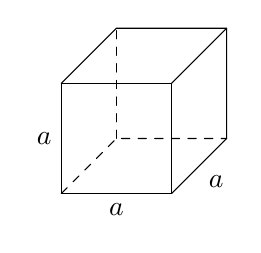
\begin{tikzpicture}[line cap=round,line join=round,>=stealth,x=0.7cm,y=0.7cm]
\draw (0,0)--(2,0)--(2,2)--(0,2)--cycle;
\draw (0,2)--(1,3)--(3,3)--(3,1)--(2,0);
\draw (2,2)--(3,3);
\draw [dashed] (0,0)--(1,1)--(3,1);
\draw [dashed] (1,1)--(1,3);
\node[below] at (1,0) {$a$};
\node[left] at (0,1) {$a$};
\node[below right] at (2.5,0.5) {$a$};
\end{tikzpicture}
\end{figurehere}
\end{center}

%kuva 35 funktio

\begin{center}
\begin{figurehere}
\begin{tikzpicture}[line cap=round,line join=round,>=triangle 45,x=0.7cm,y=0.7cm]
%x-akseli:
\draw[->,color=gray] (-2.5,0) -- (6.5,0);
%tiksut ja viivat
\foreach \x in {-2,-1,1,2,3,4,5,6}
{\draw[dashed, color= lightgray] (\x,-3.5)--(\x,7.5);
\draw[shift={(\x,0)},color=black] (0pt,1pt) -- (0pt,-1pt);
}
%\node [below] at (3.5,0) {$x$};

%y-akseli
\draw[->,color=gray] (0,-3.5) -- (0,7.5);
%tiksut ja viivat
\foreach \y in {-3,-2,-1,1,2,3,4,5,6,7}
{
\draw[dashed, color=lightgray] (-2.5,\y)--(6.5,\y);
\draw[shift={(0,\y)},color=black] (1pt,0pt) -- (-1pt,0pt);
}
%\node [left] at (0,4.5) {$y$};

% Varsinainen kuva
\draw[thick, domain=-2.5:5.45, smooth] plot (\x, {0.1875*(\x)^3-0.75*(\x)^2-0.75*(\x)+3}); 
\node[right] at (5.5,7.5) {$y = f(x)$};
%\node[right, color=blue] at (3.5,7.5) {$y = g(x)$};
%\draw (3.386,0)--(3.386,5)--(0,5);
%\draw[fill] (3.386,4.96) circle [radius=1.5pt];
%\node[below] at (3.386,0) {$a$};
%\node[left] at (0,5) {$f(a) = g(a)$};
\end{tikzpicture}
\end{figurehere}
\end{center}


%kuva 36 joki
\begin{center}
\begin{figurehere}
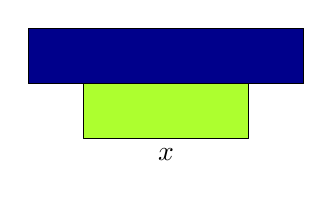
\begin{tikzpicture}[line cap=round,line join=round,>=stealth,x=0.7cm,y=0.7cm]
\draw [fill, color = DarkBlue] (0,1)--(5,1)--(5,2)--(0,2)--cycle;
\draw [fill, color = GreenYellow] (1,1)--(4,1)--(4,0)--(1,0)--cycle;
\draw (0,1)--(5,1)--(5,2)--(0,2)--cycle;
\draw (1,1)--(4,1)--(4,0)--(1,0)--cycle;
\node[below] at (2.5,0) {$x$};
\end{tikzpicture}
\end{figurehere}
\end{center}

%kuva 37 suoria

\begin{center}
\begin{figurehere}
\begin{tikzpicture}[line cap=round,line join=round,>=triangle 45,x=0.7cm,y=0.7cm]
%x-akseli:
\draw[->,color=gray] (-1.5,0) -- (4.5,0);
%tiksut ja viivat
\foreach \x in {-1,1,2,3,4}
{\draw[dashed, color= lightgray] (\x,-1.5)--(\x,4.5);
\draw[shift={(\x,0)},color=black] (0pt,1pt) -- (0pt,-1pt);
}
%\node [below] at (3.5,0) {$x$};

%y-akseli
\draw[->,color=gray] (0,-1.5) -- (0,4.5);
%tiksut ja viivat
\foreach \y in {-1,1,2,3,4}
{
\draw[dashed, color=lightgray] (-1.5,\y)--(4.5,\y);
\draw[shift={(0,\y)},color=black] (1pt,0pt) -- (-1pt,0pt);
}
%\node [left] at (0,4.5) {$y$};

% Varsinainen kuva
\draw[thick, domain=-1.5:4.5, color = green] plot (\x, {0.5*\x-0.5});
\node[right] at (4.5,1.75) {B};
\draw[thick, domain=-1.5:2.5, color = red] plot (\x, {1.5*\x+0.5});
\node[right] at (2.5,4.25) {A};
\draw[thick, domain=-1.25:1.75, color = black] plot (\x, {-2*\x+2});
\node[below] at (1.75,-1.5) {D};
\draw[thick, domain=-1.5:2.5, color = blue] plot (\x, {-1*\x+1});
\node[right] at (2.5,-1.5) {C};
\end{tikzpicture}
\end{figurehere}
\end{center}

%kuva 38 suoria

\begin{center}
\begin{figurehere}
\begin{tikzpicture}[line cap=round,line join=round,>=triangle 45,x=0.7cm,y=0.7cm]
%x-akseli:
\draw[->,color=gray] (-1.5,0) -- (4.5,0);
%tiksut ja viivat
\foreach \x in {-1,1,2,3,4}
{\draw[dashed, color= lightgray] (\x,-1.5)--(\x,4.5);
\draw[shift={(\x,0)},color=black] (0pt,1pt) -- (0pt,-1pt);
}
%\node [below] at (3.5,0) {$x$};

%y-akseli
\draw[->,color=gray] (0,-1.5) -- (0,4.5);
%tiksut ja viivat
\foreach \y in {-1,1,2,3,4}
{
\draw[dashed, color=lightgray] (-1.5,\y)--(4.5,\y);
\draw[shift={(0,\y)},color=black] (1pt,0pt) -- (-1pt,0pt);
}
%\node [left] at (0,4.5) {$y$};

% Varsinainen kuva
\draw[thick, domain=-1.5:4.5, color = green] plot (\x, {0.5*\x+0.5});
\node[right] at (4.5,2.75) {B};
\draw[thick, domain=-1.5:2.5, color = red] plot (\x, {1.5*\x+0.5});
\node[right] at (2.5,4.25) {A};
\draw[thick, domain=-1.5:1, color = black] plot (\x, {-2*\x+0.5});
\node[below] at (1,-1.5) {D};
\draw[thick, domain=-1.5:2, color = blue] plot (\x, {-1*\x+0.5});
\node[right] at (2,-1.5) {C};
\end{tikzpicture}
\end{figurehere}
\end{center}

%kuva 39 onko funktio

\begin{center}
\begin{figurehere}
\begin{tikzpicture}[line cap=round,line join=round,>=triangle 45,x=0.7cm,y=0.7cm]
%x-akseli:
\draw[->,color=gray] (-2.5,0) -- (2.5,0);
%tiksut ja viivat
\foreach \x in {-2,-1,1,2}
{\draw[dashed, color= lightgray] (\x,-2.5)--(\x,2.5);
\draw[shift={(\x,0)},color=black] (0pt,1pt) -- (0pt,-1pt);
}
%\node [below] at (3.5,0) {$x$};

%y-akseli
\draw[->,color=gray] (0,-2.5) -- (0,2.5);
%tiksut ja viivat
\foreach \y in {-2,-1,1,2}
{
\draw[dashed, color=lightgray] (-2.5,\y)--(2.5,\y);
\draw[shift={(0,\y)},color=black] (1pt,0pt) -- (-1pt,0pt);
}
%\node [left] at (0,4.5) {$y$};

% Varsinainen kuva
\draw[thick, domain=-2.1:2.1] plot (\x, {(\x)^2-2});
\node [below left] at (-2,-2) {B};
\end{tikzpicture}
\end{figurehere}
\end{center}

%kuva 40 onko funktio

\begin{center}
\begin{figurehere}
\begin{tikzpicture}[line cap=round,line join=round,>=triangle 45,x=0.7cm,y=0.7cm]
%x-akseli:
\draw[->,color=gray] (-2.5,0) -- (2.5,0);
%tiksut ja viivat
\foreach \x in {-2,-1,1,2}
{\draw[dashed, color= lightgray] (\x,-2.5)--(\x,2.5);
\draw[shift={(\x,0)},color=black] (0pt,1pt) -- (0pt,-1pt);
}
%\node [below] at (3.5,0) {$x$};

%y-akseli
\draw[->,color=gray] (0,-2.5) -- (0,2.5);
%tiksut ja viivat
\foreach \y in {-2,-1,1,2}
{
\draw[dashed, color=lightgray] (-2.5,\y)--(2.5,\y);
\draw[shift={(0,\y)},color=black] (1pt,0pt) -- (-1pt,0pt);
}
%\node [left] at (0,4.5) {$y$};

% Varsinainen kuva
\draw[thick, domain=-2:2.1, smooth, samples=200] plot (\x, {sqrt(\x+2)});
\draw[thick, domain=-2:2.1, smooth, samples=200] plot (\x, {-sqrt(\x+2)});
\node [below left] at (-2,-2) {A};
\end{tikzpicture}
\end{figurehere}
\end{center}

%kuva 41 onko funktio

\begin{center}
\begin{figurehere}
\begin{tikzpicture}[line cap=round,line join=round,>=triangle 45,x=0.7cm,y=0.7cm]
%x-akseli:
\draw[->,color=gray] (-2.5,0) -- (2.5,0);
%tiksut ja viivat
\foreach \x in {-2,-1,1,2}
{\draw[dashed, color= lightgray] (\x,-2.5)--(\x,2.5);
\draw[shift={(\x,0)},color=black] (0pt,1pt) -- (0pt,-1pt);
}
%\node [below] at (3.5,0) {$x$};

%y-akseli
\draw[->,color=gray] (0,-2.5) -- (0,2.5);
%tiksut ja viivat
\foreach \y in {-2,-1,1,2}
{
\draw[dashed, color=lightgray] (-2.5,\y)--(2.5,\y);
\draw[shift={(0,\y)},color=black] (1pt,0pt) -- (-1pt,0pt);
}
%\node [left] at (0,4.5) {$y$};

% Varsinainen kuva
\draw[thick] (0,0) circle [radius = 2];
\node [below left] at (-2,-2) {C};
\end{tikzpicture}
\end{figurehere}
\end{center}

%kuva 42 onko funktio

\begin{center}
\begin{figurehere}
\begin{tikzpicture}[line cap=round,line join=round,>=triangle 45,x=0.7cm,y=0.7cm]
%x-akseli:
\draw[->,color=gray] (-2.5,0) -- (2.5,0);
%tiksut ja viivat
\foreach \x in {-2,-1,1,2}
{\draw[dashed, color= lightgray] (\x,-2.5)--(\x,2.5);
\draw[shift={(\x,0)},color=black] (0pt,1pt) -- (0pt,-1pt);
}
%\node [below] at (3.5,0) {$x$};

%y-akseli
\draw[->,color=gray] (0,-2.5) -- (0,2.5);
%tiksut ja viivat
\foreach \y in {-2,-1,1,2}
{
\draw[dashed, color=lightgray] (-2.5,\y)--(2.5,\y);
\draw[shift={(0,\y)},color=black] (1pt,0pt) -- (-1pt,0pt);
}
%\node [left] at (0,4.5) {$y$};

% Varsinainen kuva
\draw[thick] (-2.5,1)--(2.5,1);
\node [below left] at (-2,-2) {D};
\end{tikzpicture}
\end{figurehere}
\end{center}

%kuva 43 onko funktio

\begin{center}
\begin{figurehere}
\begin{tikzpicture}[line cap=round,line join=round,>=triangle 45,x=0.7cm,y=0.7cm]
%x-akseli:
\draw[->,color=gray] (-2.5,0) -- (2.5,0);
%tiksut ja viivat
\foreach \x in {-2,-1,1,2}
{\draw[dashed, color= lightgray] (\x,-2.5)--(\x,2.5);
\draw[shift={(\x,0)},color=black] (0pt,1pt) -- (0pt,-1pt);
}
%\node [below] at (3.5,0) {$x$};

%y-akseli
\draw[->,color=gray] (0,-2.5) -- (0,2.5);
%tiksut ja viivat
\foreach \y in {-2,-1,1,2}
{
\draw[dashed, color=lightgray] (-2.5,\y)--(2.5,\y);
\draw[shift={(0,\y)},color=black] (1pt,0pt) -- (-1pt,0pt);
}
%\node [left] at (0,4.5) {$y$};

% Varsinainen kuva
\begin{scope}
\clip (-2.5,-2.5) rectangle (2.5,2.5);
\draw[thick] (-3,-2) cos (-2,0) sin (-1,2) cos (0,0) sin (1,-2) cos (2,0) sin (3,2);
\end{scope}
\node [below left] at (-2,-2) {E};

\end{tikzpicture}
\end{figurehere}
\end{center}

%kuva 44 onko funktio

\begin{center}
\begin{figurehere}
\begin{tikzpicture}[line cap=round,line join=round,>=triangle 45,x=0.7cm,y=0.7cm]
%x-akseli:
\draw[->,color=gray] (-2.5,0) -- (2.5,0);
%tiksut ja viivat
\foreach \x in {-2,-1,1,2}
{\draw[dashed, color= lightgray] (\x,-2.5)--(\x,2.5);
\draw[shift={(\x,0)},color=black] (0pt,1pt) -- (0pt,-1pt);
}
%\node [below] at (3.5,0) {$x$};

%y-akseli
\draw[->,color=gray] (0,-2.5) -- (0,2.5);
%tiksut ja viivat
\foreach \y in {-2,-1,1,2}
{
\draw[dashed, color=lightgray] (-2.5,\y)--(2.5,\y);
\draw[shift={(0,\y)},color=black] (1pt,0pt) -- (-1pt,0pt);
}
%\node [left] at (0,4.5) {$y$};

% Varsinainen kuva
\begin{scope}
\clip (-2.5,-2.5) rectangle (2.5,2.5);
\draw[thick, domain=0.1:2.5, smooth, samples=200] plot (\x, {0.4/\x});
\draw[thick, domain=-0.1:-2.5, smooth, samples=200] plot (\x, {0.4/\x});
\end{scope}
\node [below left] at (-2,-2) {F};

\end{tikzpicture}
\end{figurehere}
\end{center}

%kuva 45 leikkauspisteet

\begin{center}
\begin{figurehere}
\begin{tikzpicture}[line cap=round,line join=round,>=triangle 45,x=0.7cm,y=0.7cm]
%x-akseli:
\draw[->,color=gray] (-4.5,0) -- (4.5,0);
%tiksut ja viivat
\foreach \x in {-4,-3,-2,-1,1,2,3,4}
{\draw[dashed, color= lightgray] (\x,-3.5)--(\x,3.5);
\draw[shift={(\x,0)},color=black] (0pt,1pt) -- (0pt,-1pt);
}
%\node [below] at (3.5,0) {$x$};

%y-akseli
\draw[->,color=gray] (0,-3.5) -- (0,3.5);
%tiksut ja viivat
\foreach \y in {-3,-2,-1,1,2,3}
{
\draw[dashed, color=lightgray] (-4.5,\y)--(4.5,\y);
\draw[shift={(0,\y)},color=black] (1pt,0pt) -- (-1pt,0pt);
}
%\node [left] at (0,4.5) {$y$};

% Varsinainen kuva
\begin{scope}
\clip (-4.5,-3.5) rectangle (4.5,3.5);
\draw[thick, domain=-4.5:4.5, smooth, samples=200, color = blue] plot (\x, {-0.25*(\x)^2+2});
\draw[thick, domain=-4.5:4.5, smooth, samples=200] plot (\x, {0.5*\x});
\end{scope}
\node [right] at (4.5,-3) {\textcolor{blue}{$y = g(x)$}};
\node [right] at (4.5,2.2) {\textcolor{black}{$y = f(x)$}};
\end{tikzpicture}
\end{figurehere}
\end{center}

%kuva 46 koordinaatisto

\begin{center}
\begin{figurehere}
\begin{tikzpicture}[line cap=round,line join=round,>=triangle 45,x=0.5cm,y=0.5cm]
%x-akseli:
\draw[->,color=gray] (-6.5,0) -- (6.5,0);
%tiksut ja viivat
\foreach \x in {-6,-5,-4,-3,-2,-1,1,2,3,4,5,6}
{\draw[dashed, color= lightgray] (\x,-6.5)--(\x,6.5);
\draw[shift={(\x,0)},color=black] (0pt,1pt) -- (0pt,-1pt);
}
%\node [below] at (3.5,0) {$x$};

%y-akseli
\draw[->,color=gray] (0,-6.5) -- (0,6.5);
%tiksut ja viivat
\foreach \y in {-6,-5,-4,-3,-2,-1,1,2,3,4,5,6}
{
\draw[dashed, color=lightgray] (-6.5,\y)--(6.5,\y);
\draw[shift={(0,\y)},color=black] (1pt,0pt) -- (-1pt,0pt);
}
%\node [left] at (0,4.5) {$y$};

% Varsinainen kuva
%\begin{scope}
%\clip (-4.5,-3.5) rectangle (4.5,3.5);
%\draw[thick, domain=-4.5:4.5, smooth, samples=200, color = blue] plot (\x, {-0.25*(\x)^2+2});
%\draw[thick, domain=-4.5:4.5, smooth, samples=200] plot (\x, {0.5*\x});
%\end{scope}
%\node [right] at (4.5,-3) {\textcolor{blue}{$y = g(x)$}};
%\node [right] at (4.5,2.2) {\textcolor{black}{$y = f(x)$}};
\end{tikzpicture}
\end{figurehere}
\end{center}